%$Header: /home/dashley/cvsrep/e3ft_gpl01/e3ft_gpl01/dtaipubs/cron/2006/phdtopicpropa/phdtopicpropa.tex,v 1.20 2006/03/27 00:10:30 dashley Exp $
\documentclass[letterpaper,10pt,titlepage]{article}
%
%\pagestyle{headings}
%
\usepackage{amsmath}
\usepackage{amsfonts}
\usepackage{amssymb}
\usepackage[ansinew]{inputenc}
\usepackage[OT1]{fontenc}
\usepackage{graphicx}
%
\begin{document}
%-----------------------------------------------------------------------------------
\title{Ph.D. Topic Proposal}
\author{\vspace{2cm}\\David T. Ashley\\\texttt{dta@e3ft.com}\\\vspace{2cm}}
\date{\vspace*{8mm}\small{Version Control $ $Revision: 1.20 $ $ \\
      Version Control $ $Date: 2006/03/27 00:10:30 $ $ (UTC) \\
      $ $RCSfile: phdtopicpropa.tex,v $ $ \\
      \LaTeX{} Compilation Date: \today{}}}
\maketitle

%%%%%%%%%%%%%%%%%%%%%%%%%%%%%%%%%%%%%%%%%%%%%%%%%%%%%%%%%%%%%%%%%%%%%%%%%%%%%%%
%
\begin{abstract}
This document describes my Ph.D. research interests and provides
supporting information.  The interests
(described in \S{}\ref{srin0}) revolve around the mathematical
basis of timed automata systems and code generation
from timed automata models. 
\end{abstract}

\clearpage{}
\pagenumbering{roman}    %No page number on table of contents.
\tableofcontents{}
\clearpage{}
\listoffigures
\clearpage{}

%%%%%%%%%%%%%%%%%%%%%%%%%%%%%%%%%%%%%%%%%%%%%%%%%%%%%%%%%%%%%%%%%%%%%%%%%%%%%%%
%Force the page number to 1.  We don't want to number the table of contents
%page.
%
\setcounter{page}{1}
\pagenumbering{arabic}
%%%%%%%%%%%%%%%%%%%%%%%%%%%%%%%%%%%%%%%%%%%%%%%%%%%%%%%%%%%%%%%%%%%%%%%%%%%%%%%

\section{The Timed Automata Framework}
\label{staf0}

The framework of timed automata isn't commonplace in electrical
engineering, so this section provides 
a description.


%%%%%%%%%%%%%%%%%%%%%%%%%%%%%%%%%%%%%%%%%%%%%%%%%%%%%%%%%%%%%%%%%%%%%%%%%%%%%%%

\subsection{The Framework}
\label{staf0:stfw0}

The formal framework of timed automata consists of systems of 
automatons, each with discrete states, transitions, and
timers that can be reset to zero on transitions.

The framework includes synchronization mechanisms between automatons (i.e.
automatons may interact in well-defined ways)\@. Synchronization mechanisms 
consist of ``soft'' synchronization mechanisms and ``hard'' synchronization
mechanisms.

\begin{itemize}
\item \emph{Soft} synchronization mechanisms involve one automaton having transition
      functions that involve the discrete state or timers of another automaton.
\item \emph{Hard} synchronization mechanisms involve events.  The semantics 
      of an event require two or more
      automatons to make corresponding transitions at exactly the same time.
\end{itemize}

The details of the framework aren't especially important, 
and there are several 
variations on the framework\footnote{Variations include
substates, differences in the semantics of events, and dynamics that go beyond
$\dot{t} = 1$ (i.e. hybrid systems).} that don't change the essential properties.

The essential properties of the framework (that don't change with the variations) are:

\begin{itemize}
\item A system of timed automata that interact via synchronization
      mechanisms can be mathematically combined into a single
      larger automaton with a single
      discrete state space.
\item There is some symbolic method of reasoning about what values 
      timers can attain in each discrete state (polytopes, DBMs, etc.).
\item The symbolic reasoning about timer values often allows reasoning about
      properties of the system (reachability, liveness, etc.).
\end{itemize}

Timed automata are recognizeable to any embedded software engineer as 
``state machines''.  A typical automotive embedded system consists of many 
features and software components involving discrete state.  For example, 
software to control an automobile drivetrain with features like automatic 4-wheel drive
as well as sensor and actuator failure modes tends to have a very large discrete
space.

As a contrived example of a system of timed automata, consider the problem of 
controlling a drawbridge with one motor and two limit switches so that it goes up and down 
with period $K_D + K_U$ (Fig. \ref{fig:staf0:stfw0:000}).

\begin{figure}
\centering
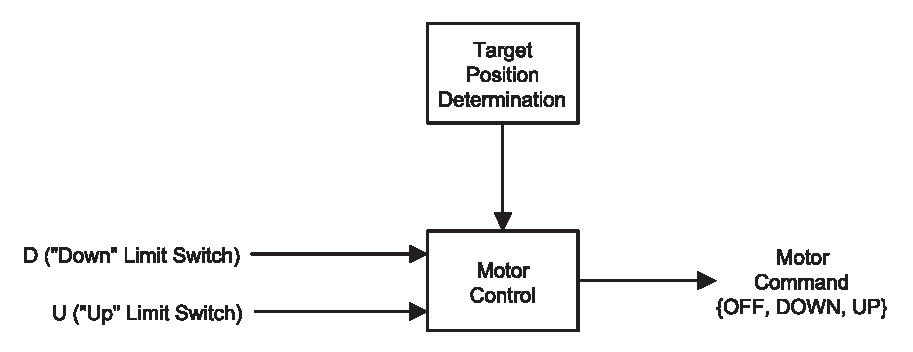
\includegraphics[width=4.0in]{system01.eps}
\caption{Example Timed Automata System (Drawbridge Control)}
\label{fig:staf0:stfw0:000}
\end{figure}

Assume that when raising the drawbridge, it is adequate to energize the motor 
until the limit switch $U$ closes.  However, when closing the drawbridge,
it is necessary to energize the motor for time $K_L$ beyond 
when the limit switch $D$ closes (the $B_{DOWNLOCK}$ state in 
Fig. \ref{fig:staf0:stfw0:01}).

One way to design such a system is with two automata
(Fig. \ref{fig:staf0:stfw0:00} and Fig. \ref{fig:staf0:stfw0:01}) interacting via
synchronization mechnisms.

The automaton of Fig. \ref{fig:staf0:stfw0:00} alternates between two
states with period $K_D + K_U$.  At any point in time, the state of this
automaton indicates whether the drawbridge should be down or up.

\begin{figure}
\centering
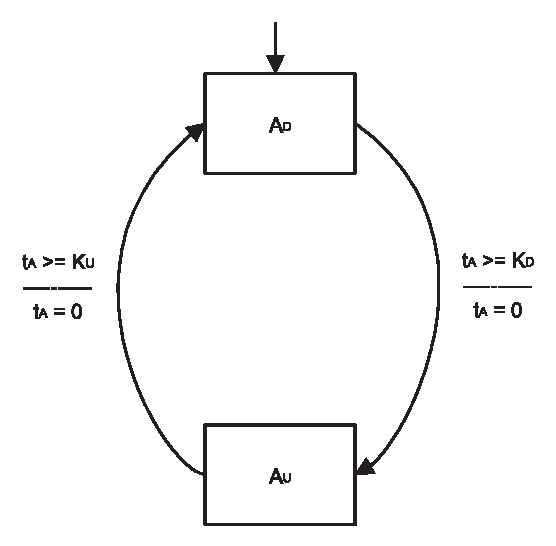
\includegraphics[height=2.5in]{exta01.eps}
\caption{Example Timed Automaton (Drawbridge Target Position Determination)}
\label{fig:staf0:stfw0:00}
\end{figure}

The automaton of Fig. \ref{fig:staf0:stfw0:01} directly
determines the energization of the bridge motor as a function of 
the limit switches $D$ and $U$, the discrete state of the automaton
of Fig. \ref{fig:staf0:stfw0:00}, and time.
In the $B_{IDLE}$ state, the motor is deenergized.
In the $B_{UP}$ state, the motor is energized to move the
drawbridge up.  In the $B_{DOWN}$ and $B_{DOWNLOCK}$ states,
the motor is energized to move the drawbridge down.

\begin{figure}
\centering
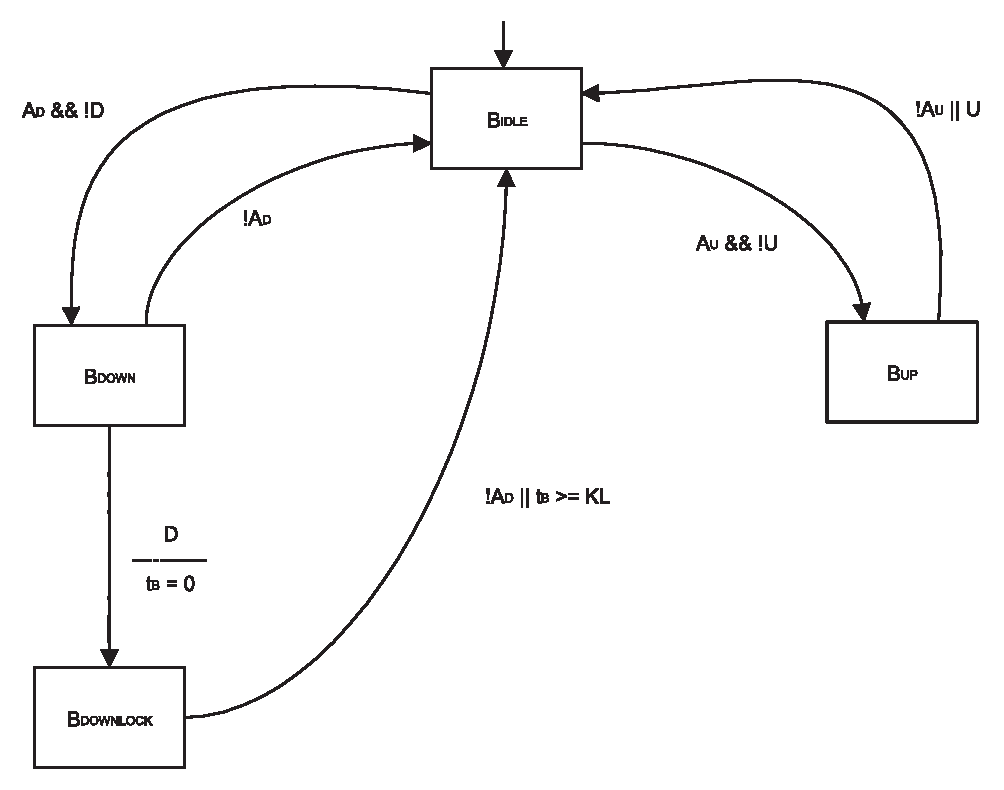
\includegraphics[width=4.6in]{exta02.eps}
\caption{Example Timed Automaton (Drawbridge Motor Control)}
\label{fig:staf0:stfw0:01}
\end{figure}

Mathematically, the automata of Figs. 
\ref{fig:staf0:stfw0:00}
and
\ref{fig:staf0:stfw0:01} can be combined to give the automaton of
Fig. \ref{fig:staf0:stfw0:02}\@.  This mathematical operation is sometimes called the
``shuffle'' operation.

\begin{figure}
\centering
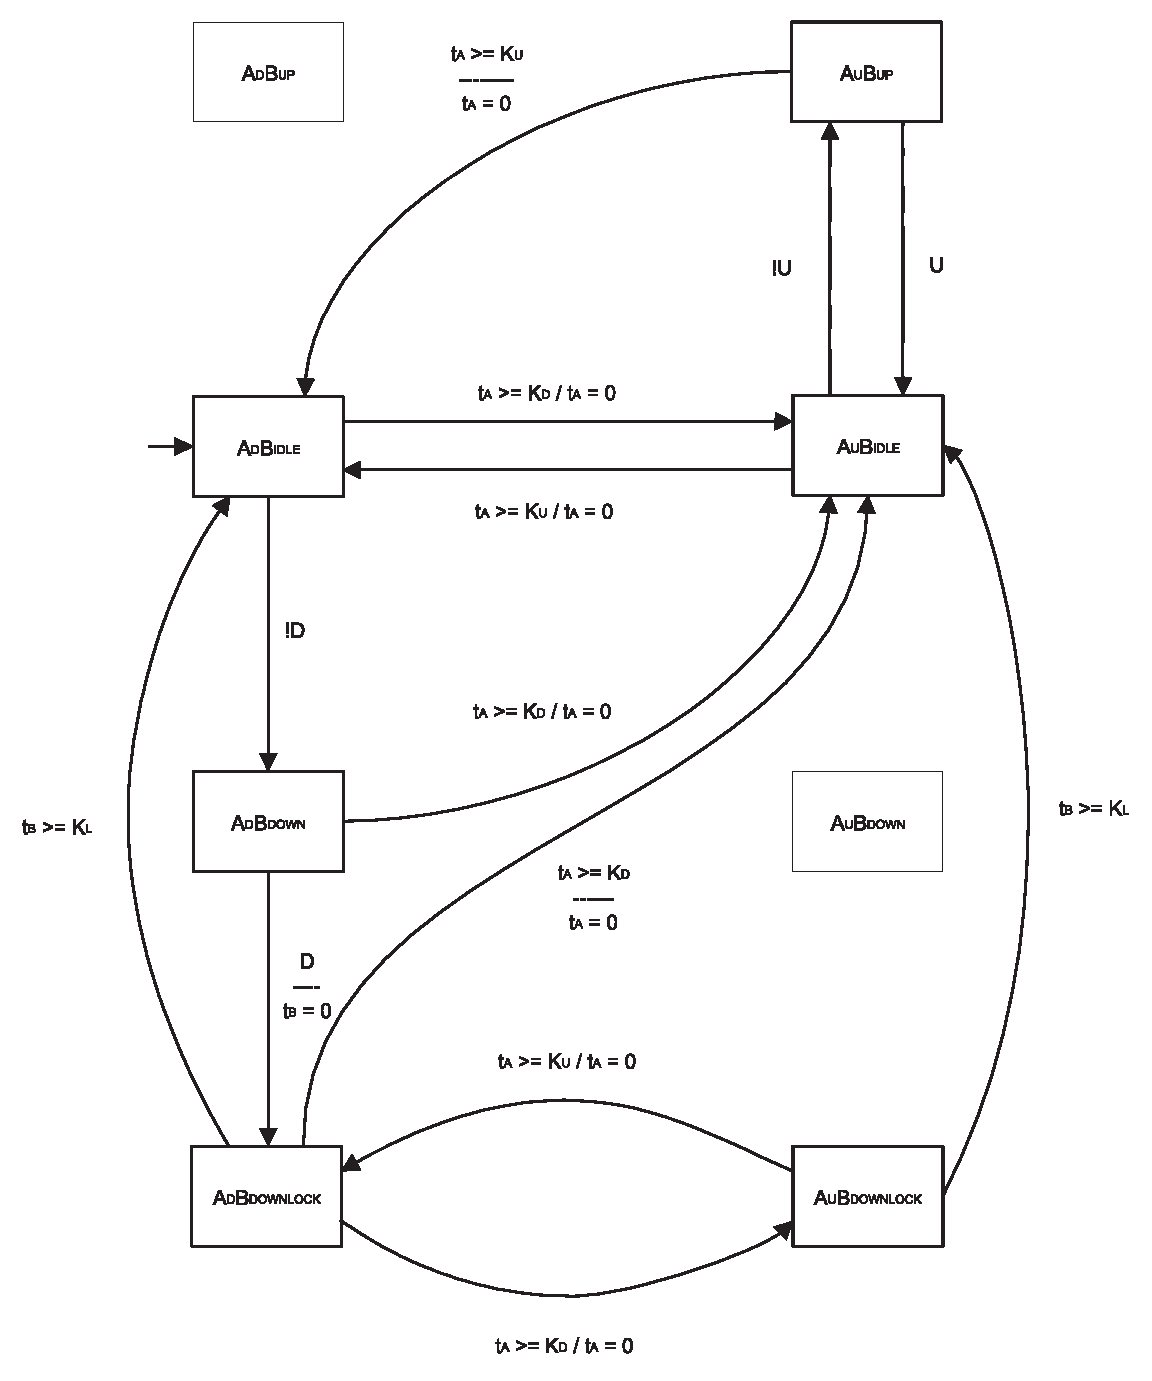
\includegraphics[width=4.6in]{exta03.eps}
\caption{Example Timed Automaton (Shuffle of Fig. \ref{fig:staf0:stfw0:00} and Fig. \ref{fig:staf0:stfw0:01})}
\label{fig:staf0:stfw0:02}
\end{figure}

In Fig. \ref{fig:staf0:stfw0:02}, each of the eight discrete states
corresponds to one discrete state from Fig. \ref{fig:staf0:stfw0:00}
and one discrete state from In Fig. \ref{fig:staf0:stfw0:01}.
The initial state $A_{D}B_{IDLE}$ corresponds to the initial state
from In Fig. \ref{fig:staf0:stfw0:00} paired with the initial state
from Fig. \ref{fig:staf0:stfw0:01}.

The noteworthy features of Fig. \ref{fig:staf0:stfw0:02} are:

\begin{itemize}
\item It is the result of a mathematical algorithm applied to 
      Figs. \ref{fig:staf0:stfw0:00} and \ref{fig:staf0:stfw0:01}.
      If the underlying system consisted of more than two automata, the
      algorithm could be applied repeatedly to generate a single automaton with
      a single large discrete state space.
\item The upper bound on the number of discrete states in the shuffle
      of two automata is the product of the number of discrete states
      in each.  Note, however, that $A_{D}B_{UP}$ and $A_{U}B_{DOWN}$
      don't ``truly'' exist.  The reason is that the synchronization
      mechanisms between the two automata ensure that these states
      are instantly exited as soon as they are entered.  Thus, a system
      of equivalent functionality can be constructed with six discrete
      states rather than eight.
\end{itemize}

Although the preceding example is contrived, it illustrates the flavor
of the framework and how separate automata with synchronization mechanisms can be
combined (and perhaps also ``separated'' or ``factored'', \S{}\ref{srin0:star0}).

It should also be apparent that tools can verify a great deal about
the system through symbolic manipulation.  Properties that can be verified
include:

\begin{itemize}
\item \emph{Reachability:} it can be symbolically determined whether
      or not each state is reachable (the algorithms involve determining
      symbolically which values timers can achieve in each discrete state and
      comparing that information against transition functions---some transitions
      cannot ever be taken).
\item \emph{Liveness:} it can be symbolically determined whether the system
      can enter a state where no inputs to the system can cause all of a
      set of states to be reachable.
\end{itemize}

The example comes \emph{very} close to the way practical
software systems are constructed.  Generally, state machines in 
software have transition functions that involve time and the states of
other state machines.


%%%%%%%%%%%%%%%%%%%%%%%%%%%%%%%%%%%%%%%%%%%%%%%%%%%%%%%%%%%%%%%%%%%%%%%%%%%%%%%

\subsection{Human Tendencies}
\label{staf0:shtd0}

My experience in industry is that human beings do badly with the
design of stateful controllers.  Typical tendencies:

\begin{itemize}
\item \textbf{Bloating of the controller state space:}
      \;It is very common for engineers to design a controller with
      a discrete state space that is too large.  The prototypical
      example is an engineer who finds a way to implement a purely combinational
      function using sequential logic.

      In the most humorous case (purely combinational logic implemented as
      sequential logic), 
      the system usually behaves correctly.  Serious software defects
      most typically come about through \emph{subtle} design mistakes.  A typical software defect
      involves two or more software components with some interaction that enter
      states such that the software can't recover.
\item \textbf{Inability to comprehend all possible behaviors of the system:}
      Very stateful systems tend to be incompatible with human cognitive
      ability.  Even when the problem is well-defined and when the controller and
      plant are operating perfectly, human beings don't do
      well at considering every possible behavior.
\item \textbf{Inability to comprehend how the system may behave in the presence
      of failures:}
      Very stateful systems are often designed to be tolerant of certain types
      of sensor and actuator failures (usually in the sense that the failures will
      be detected and the system will employ a different algorithm to operate without
      a specific sensor or actuator)\@.  Such fault detection and tolerance
      normally complicates the software design substantially.

      However, even without designed-in fault tolerance, there is the need to
      design controllers to tolerate the faults that can occur in any practical system.
      Specific scenarios that must be tolerated:

      \begin{itemize}
      \item Spurious reset of the controller (which will normally reset the controller
            to its initial state but leave the plant undisturbed).  (This directly implies that
            the system must recover from the initial state of the controller combined with
            any state of the plant.)
      \item State upset of the controller (due to electrical noise, internal software errors,
            etc.).  (This directly implies that the system must recover from any state of
            the controller combined with any state of the plant.)
      \end{itemize}

      Except in simple cases, human beings don't have the cognitive capacity to consider
      all possible behaviors when both the controller and the plant may start in any state.
\end{itemize}

One example that comes to mind from product development is an automobile transfer case controller
where it was discovered that if the electrical connector was removed, the transfer case mechanical
components repositioned, and the electrical connection restored; the controller would not
recover into normal operation.  Human beings are not good at mentally exploring all possibilities, and even
a disciplined manual process can't be used because the combinations sometimes number in the thousands
or more.  A mathematical framework and tool support are required.


%%%%%%%%%%%%%%%%%%%%%%%%%%%%%%%%%%%%%%%%%%%%%%%%%%%%%%%%%%%%%%%%%%%%%%%%%%%%%%%

\subsection{Code Generation}
\label{staf0:scgn0}

In most engineering environments, software is generated
from software designs that involve timed automata.  (Some of the techniques
used to create compact code are described in \S{}\ref{sfrr0}.)

For some types of systems, there has been success in using
existing tools to generate code directly from the software design
(using tool chains from \emph{The Math Works} or \emph{I-Logix}).  It is,
however, known from experience that a clever human programmer can generate
more compact code than any existing tool; so code generation tools have
not penetrated cost-sensitive automotive products involving 32K of FLASH or less.

There are two primary arguments against manual generation of code:

\begin{itemize}
\item Code is redundant with respect to a software design.
      In general, it does not make economic sense to maintain redundant
      information using human labor.
\item The act of optimizing implementations typically destroys the
      clear relationship between design and code.  Furthermore, changes
      to the design---sometimes even small ones---can invalidate the
      mathematical basis for certain optimizations.  Optimized code becomes
      unmaintainable.  It would be more economical to evaluate the viability 
      of optimizations and to generate code using software tools (rather than
      human labor).
\end{itemize}


%%%%%%%%%%%%%%%%%%%%%%%%%%%%%%%%%%%%%%%%%%%%%%%%%%%%%%%%%%%%%%%%%%%%%%%%%%%%%%%

\subsection{Formal Verification of Properties}
\label{staf0:svpr0}

Typical design tools provide simulation capability, and there is a large
body of theory and best practice about how to design test cases based on
a stateful design.

Still, the following problems remain:

\begin{itemize}
\item Systems with a large discrete state space elude human
      understanding.
\item It is very laborious to test systems with a large discrete
      state space.
\item It isn't possible to fully test systems with a large
      discrete state space.
\item It is possible (and common) to make a good faith effort at 
      comprehensively testing systems but still to overlook
      unacceptable behavior.
\end{itemize}

\emph{Simulation and testing are not enough.}  For complex safety-critical
systems, simulation and testing do not provide enough assurance about the
behavior of the system.

Formal verification of properties would involve making mathematical assertions
about how the system must and must not behave, and then allowing
tools to verify the properties.

Possible types of properties:

\begin{itemize}
\item \emph{Required behavior:}
      For example:  \emph{When the brake pedal switch is closed,
      the brake lights must always come on within 200ms.}
\item \emph{Required absence of behavior:}
      For example:  \emph{The airbags can never deploy without at least one
      body deformation sensor indicating body deformation.}
\item \emph{Liveness:}
      For example:  \emph{A certain set of states is always reachable by manipulating certain
      inputs.}
\end{itemize}

The only tool I'm aware of that allows formal verification of properties
is UPPAAL.  However, the modeling framework of 
UPPAAL isn't rich enough to support practical embedded systems.\footnote{The
tool chains from \emph{The Math Works} and \emph{I-Logix} don't attempt
formal verification at all.}

I would tend to view formal verification of properties as a last line of defense
against egregious software defects (i.e. as a practice that cannot stand alone)\@.  
Formal verification should be combined with all other known
best practices.


%%%%%%%%%%%%%%%%%%%%%%%%%%%%%%%%%%%%%%%%%%%%%%%%%%%%%%%%%%%%%%%%%%%%%%%%%%%%%%%

\section{FLASH/ROM Reduction Techniques}
\label{sfrr0}

In this section, I mention some of the FLASH/ROM reduction techniques
used by human programmers.  Important points:

\begin{itemize}
\item All of the techniques have a mathematical basis.
\item The techniques are complex to apply and best carried out by tools.
\item The mathematical basis of the techniques is non-trivial.  There are
      many unexplored corners.
\item The techniques distort the correspondence (i.e. the resemblance)
      between design and code, and make code unmaintainable (it would be
      better only to generate code from designs and never to maintain
      code directly).
\end{itemize}

The list of techniques presented is not exhaustive (far more techniques
exist).

%%%%%%%%%%%%%%%%%%%%%%%%%%%%%%%%%%%%%%%%%%%%%%%%%%%%%%%%%%%%%%%%%%%%%%%%%%%%%%%

\subsection{General Paradigm of Software Construction for Small Microcontrollers}
\label{sfrr0:sgsc0}

This discussion is confined entirely to systems where a stateful design is
implemented directly as code (with no tabulation or compression of the design).
Other paradigms are possible.  For example, at least one tool on the market implements
stateful designs as state transition tables that are evaluated at runtime by
a table interpreter.  My experience with these types of systems is that there 
is always a real-time performance penalty (but certainly not always a
FLASH penalty).  My research interests do also include event-driven systems
and systems where the design is not implemented directly as code; but these
systems are not mentioned for brevity.

The most common paradigm for small systems is ``\emph{a collection of cooperating
timed automatons}''.  The most typical abstraction of these systems is a data-flow
diagram, with RAM variables (i.e. global variables) used as the interfaces.

There is a body of theory and best practice about what separates good software designs
and implementations from bad (Parnas and the classic coupling and cohesion spectrums
come to mind).  However, in small systems, it simply isn't possible to
implement the systems using classic ``good'' programming practice---formal parameters,
pointer dereferencing, and access to variables in stack frames all bloat
FLASH size under the weak instruction sets typical of small microcontrollers.

It is helpful to take a step back and consider the possibility that global variables
(the second-strongest form of coupling in the classic coupling spectrum) aren't
inherently harmful; but rather that it is the way in which global variables are
typically used that causes harm.  The harmful aspects of global variables
seem to be:

\begin{itemize}
\item If global variables are tested \emph{and assigned} in more than place,
      the variable actually becomes an automaton and adds to the
      state space of the system.
\item Global variables lead to unrestrained connectivity:  \emph{any}
      software component can access the variables.  Additionally,
      state is not ``shed'' as functions return (as happens with formal
      parameters and local variables)\@.  This leads to connectivity
      that often skips levels of the calling tree (making it very
      difficult to understand the software).
\end{itemize}

Small systems often have design rules to mitigate the harmful aspects of
global variables.  The design rules tend to involve these restrictions:

\begin{itemize}
\item A global variable used as an interface can be assigned by only one
      software component (a 1-writer, $n$-reader restriction).
\item A global variable used as an interface has its readers/writers
      represented in design documentation (so that the connectivity
      created by the global variable isn't accidental or unrestrained).
\end{itemize}

The design rules typically also include provisions for global variables
used as interfaces that are tested and assigned by more than one software
component (i.e. interface automatons).  The simplest example of such an 
interface is a semaphore that is
set \emph{T} by one software component and tested and set \emph{F} by
another software component, but the design rules are far more general.

Note that tools can be used to allow a system to be phrased in a way
consistent with the traditional coupling spectrum but implemented 
efficiently for small microcontrollers.  For example, some compilers 
are able to analyze the calling tree and place variables of storage 
class \emph{automatic} into statically overlaid\footnote{Statically overlaid
based on the calling tree:  one function's automatic variables can be overlaid
with another only if an analysis of the calling tree determines that 
the two functions cannot be active at the same time.} areas of memory rather than
in a stack frame.  Similar tool support could be developed for the notion of
\emph{automatic} bitfields and to restrain the connectivity introduced
by global variables to be consistent with the product design.


%%%%%%%%%%%%%%%%%%%%%%%%%%%%%%%%%%%%%%%%%%%%%%%%%%%%%%%%%%%%%%%%%%%%%%%%%%%%%%%

\subsection{Near versus Far (Addressing Modes)}
\label{sfrr0:snvf0}

Most small microcontrollers (TMS370C8, 68HC05, etc.) have two 
non-indexed addressing modes, typically called \emph{direct} and
\emph{extended}.  Instructions using the direct addressing mode typically
have the address encoded as a single byte, and can address only locations
\$00 through \$FF\@.  Instructions using the extended addressing mode
typically have the address encoded as two bytes, and can address
locations \$0000 through \$FFFF.

For lack of better nomenclature, I'll call the RAM locations that can be addressed
using short instructions \emph{near} RAM, and the RAM locations that require
long instructions \emph{far} RAM.

When fixed RAM locations are used as interfaces (\S{}\ref{sfrr0:sgsc0}),
one can save substantial FLASH by allocating the variables that are 
referenced most often throughout the software into near RAM.

In automotive software, variables such as gearshift position and vehicle speed
are typically referenced many times throughout FLASH.  Most programmers
would automatically place these into near RAM.

However, for most variables, it isn't obvious whether these should be placed
into near or far RAM.

Software developers often write small utility programs to scan all software
modules to determine the number of references to each variable.  This information
is then used to allocate the variables with the most references into near RAM.

The FLASH savings from using this technique is typically large.  As an example,
assume there are ten variables each referenced 50 times throughout the software.
The savings of placing these variables into near RAM versus far RAM is
typically about $50 \times 10 = 500$ bytes of FLASH (more than 1\% of a
32K FLASH).


%%%%%%%%%%%%%%%%%%%%%%%%%%%%%%%%%%%%%%%%%%%%%%%%%%%%%%%%%%%%%%%%%%%%%%%%%%%%%%%

\subsection{Treatment of Time}
\label{sfrr0:stot0}

The way that time is measured is usually the single most important decision
in a small embedded system.  Typically, many software components have to 
measure time intervals, so a suboptimal decision about the mechanisms
greatly increases FLASH consumption.

The best mechanism known is to arrange all software timers into
binary decades and to decrement the timers en masse
(Fig. \ref{fig:sfrr0:stot0:00}).

\begin{figure}
\begin{small}
\begin{verbatim}
unsigned char modulo_counter;
unsigned char timers_modulo_1[MOD1_COUNT];
unsigned char timers_modulo_2[MOD2_COUNT];
unsigned char timers_modulo_4[MOD4_COUNT];

void decrement_timers(void)
   {
   int i;

   modulo_counter++;

   for (i=0; i<sizeof(timers_modulo_1)/sizeof(timers_modulo_1[0]); i++)
      {
      if (timers_modulo_1[i])
         timers_modulo_1[i]--;
      }

   if (modulo_counter & 0x01)
      {
      for (i=0; i<sizeof(timers_modulo_2)/sizeof(timers_modulo_2[0]); i++)
         {
         if (timers_modulo_2[i])
            timers_modulo_2[i]--;
         }
      }

   if (modulo_counter & 0x02)
      {
      for (i=0; i<sizeof(timers_modulo_4)/sizeof(timers_modulo_4[0]); i++)
         {
         if (timers_modulo_4[i])
            timers_modulo_4[i]--;
         }
      }
   }
\end{verbatim}
\end{small}
\caption{Software Timers Decremented En Masse}
\label{fig:sfrr0:stot0:00}
\end{figure}

When software components must measure time, a byte
(\texttt{timers\_modulo\_4[2]}, for example) is set to a non-zero value.
A separate software component, usually resembling Fig. \ref{fig:sfrr0:stot0:00} but often
implemented in assembly-language,
decrements the byte, but not below zero.
A test against zero will determine if the time period has expired.

The single-byte mechanism combined with binary decades allows any time period
to be measured within 1:128.  For example, assume that the binary decades are
$2^q \times 1ms$ (1ms, 2ms, 4ms, etc.) and then that
we wish to measure a time period of 30 minutes.  Then

\begin{equation}
255 (2^q) \geq 1,800,000
\end{equation}

\begin{equation}
q = \left\lceil \log_2 \frac{1,800,000}{255} \right\rceil = 13
\end{equation}

A timer resolution of $2^{13} = 8,192$ms with a count of 219 or 220 would in practice be used.
For most automotive applications, measuring 30 minutes within 8 seconds is acceptable.

It is noteworthy that using coarse software timers introduces nondeterminism
into the system (although I've never seen a problem in practice) and probably requires
some adjustment to timed automata algorithms used for verification of properties.


%%%%%%%%%%%%%%%%%%%%%%%%%%%%%%%%%%%%%%%%%%%%%%%%%%%%%%%%%%%%%%%%%%%%%%%%%%%%%%%

\subsection{Bitfields of Size One}
\label{sfrr0:sbfi0}

Many small microcontrollers possess extremely efficient instructions
for clearing, setting, and testing individual bits of RAM (especially near
bits).  It isn't uncommon for a microcontroller to have an instruction that
will test a bit and conditionally branch.

Note that economies apply only to bitfields of size one.  Bitfields of
other sizes require the compiler to mask and shift to obtain the value of the
bitfield, then to shift and mask to store the value back.

The economy of bitfields of size one has several implications for the construction 
of embedded software.

\begin{itemize}
\item Variables that are conceptually Boolean should never be
      maintained as full bytes.  Bitfields are more efficient, both
      in FLASH and RAM.
\item In many cases, it is most efficient to maintain discrete state as
      bitfields rather than as a byte.  A state machine with three
      discrete states is often most effectively implemented as two
      bitfields with state assignments 0/0, 0/1, and 1/X.
\item It is often most effective to evaluate common Boolean subexpressions and store
      the results in bitfields (\S{}\ref{sfrr0:scse0}).
\end{itemize}


%%%%%%%%%%%%%%%%%%%%%%%%%%%%%%%%%%%%%%%%%%%%%%%%%%%%%%%%%%%%%%%%%%%%%%%%%%%%%%%

\subsection{Equivalence Classing of Discrete States}
\label{sfrr0:secd0}

The most obvious way to construct a state machine in software is shown in
Fig. \ref{fig:sfrr0:secd0:00}.  Discrete state is maintained
as a byte, and each state has a value $\in \{0, \ldots{}, 255\}$.

\begin{figure}
\begin{small}
\begin{verbatim}
switch (state)
   {
   default:
   case 0:
      {
      if (some_transition_condition)
         {
         state = 1;
         }
      break;
      }
   case 1:
      {
      if (some_other_transition_condition)
         {
         state = 0;
         }
      break;
      }
   case 2:
      {
      ...
      break;
      }
   }
\end{verbatim}
\end{small}
\caption{Most Obvious Construction of State Machine in Software}
\label{fig:sfrr0:secd0:00}
\end{figure}

The shortcoming of the approach shown in Fig. \ref{fig:sfrr0:secd0:00} is that
state machines are often accompanied by:

\begin{itemize}
\item Combinational logic that implements combinational functions involving
      the discrete state of the state machine being considered.
\item Transition functions in other state machines that depend on the discrete
      state of the state machine being considered.
\end{itemize}


\begin{figure}
\begin{small}
\begin{verbatim}
if (
        (state == 0)  || (state == 13) || (state == 18) || (state == 30)
     || (state == 31) || (state == 51) || (state == 99)
   ) 
\end{verbatim}
\end{small}
\caption{Typical Test for Membership in a Set of Discrete States}
\label{fig:sfrr0:secd0:01}
\end{figure}

This can often lead to tests of the form shown in
Fig. \ref{fig:sfrr0:secd0:01}.
Such tests are very expensive, both in FLASH consumption and in execution time.
A typical compiler must generate many compare instructions.

One can make the observation that there are many machine instructions that
create equivalence classes within $\mathbb{Z}^+$:

\begin{itemize}
\item An \emph{AND \#1} instruction may create equivalence classes such as 
      \{0, 2, 4, \ldots{}\} versus \{1, 3, 5, \ldots{}\}.  Other \emph{AND} instructions
      can create more complex equivalence classes.
\item A \emph{CMP \#n} instruction usually creates three equivalence classes:  the integers less than $n$,
      $n$, and the integers greater than $n$.
\item There are other machine instructions that create different equivalence classes.
\end{itemize}

The critical question is whether one can assign discrete state values so as to
make the best utilization of the equivalence classes that machine instructions
naturally create.  For example, if a test for 10 distinct discrete states occurs
many places in the software, it would make sense to try to assign these
state values so that they are part of an equivalence class that can be
identified immediately by one or two machine instructions.

It should be obvious that if many different tests of discrete state are involved,
identifying an optimal or near-optimal assignment of discrete state values and
the accompanying tests would be very difficult to do by hand.  This type of
optimization is best done by software tools.


%%%%%%%%%%%%%%%%%%%%%%%%%%%%%%%%%%%%%%%%%%%%%%%%%%%%%%%%%%%%%%%%%%%%%%%%%%%%%%%

\subsection{Ordering of Transition Functions}
\label{sfrr0:sotf0}

It often happens that transition functions have common subexpressions.
For example, consider the code snippet in Fig. \ref{fig:sfrr0:sotf0:00}.
The subexpression ``\texttt{A \&\& B}'' is common to both transitions
out of State 0. 

\begin{figure}
\begin{small}
\begin{verbatim}
switch (state)
   {
   default:
   case 0:
      {
      if (A && B && C)
         {
         state = 1;
         }
      else if (A && B && !D)
         {
         state = 2;
         }
      break;
      }
   case 1:
      {
      ...
      break;
      }
   case 2:
      {
      ...
      break;
      }
   }
\end{verbatim}
\end{small}
\caption{State Machine Before Control Flow Removal of Common Subexpression}
\label{fig:sfrr0:sotf0:00}
\end{figure}

The code can be optimized to evaluate this subexpression only once
(Fig. \ref{fig:sfrr0:sotf0:01}).

\begin{figure}
\begin{small}
\begin{verbatim}
switch (state)
   {
   default:
   case 0:
      {
      if (A && B)
         {
         if (C)
            {
            state = 1;
            }
         else if (!D)
            {
            state = 2;
            }
         }
      break;
      }
   case 1:
      {
      ...
      break;
      }
   case 2:
      {
      ...
      break;
      }
   }
\end{verbatim}
\end{small}
\caption{State Machine After Control Flow Removal of Common Subexpression}
\label{fig:sfrr0:sotf0:01}
\end{figure}

In the trivial case presented, it is easy to identify the subexpression
and rearrange the code so that it is evaluated only once.  However, more complex cases
involve logical implication; i.e. there is not an identifiable subexpression, but there
is still a way to rearrange the code for better efficiency.  Such analysis is
best done by software tools.


%%%%%%%%%%%%%%%%%%%%%%%%%%%%%%%%%%%%%%%%%%%%%%%%%%%%%%%%%%%%%%%%%%%%%%%%%%%%%%%

\subsection{Common Subexpression Elimination}
\label{sfrr0:scse0}

It often occurs that the same subexpression appears in transition functions from
more than one discrete state.  It can be economical to rearrange the 
code to evaluate such subexpressions
only once.  Two approaches occur in practice:

\begin{itemize}
\item The subexpression is evaluated once, regardless of discrete state, and the
      result is placed in a temporary variable (often a bitfield if the expression
      has a Boolean result).
\item The evaluation of the subexpression is implemented as a subroutine, and
      the subroutine is called from more than one transition function.
\end{itemize}

Each of these two approaches has advantages and disadvantages.

Identifying common subexpressions and deciding how to eliminate the FLASH
penalty associated with duplicated code is a tedious task and best done
by software tools.

%%%%%%%%%%%%%%%%%%%%%%%%%%%%%%%%%%%%%%%%%%%%%%%%%%%%%%%%%%%%%%%%%%%%%%%%%%%%%%%

\subsection{Farey Series Approximations}
\label{sfrr0:sfsa0}

Many modern microcontrollers have an efficient integer multiplication
instruction, and some also have an efficient integer division instruction.
Fixed-point arithmetic is the norm in small microcontroller work, and it
is common to want to approximate functions of the form

\begin{equation}
y = r_I x
\end{equation}

\noindent{}with $r_I \in \mathbb{R}^+$ and $x,y \in \mathbb{Z}^+$.  $r_I$ is the
``ideal'' scaling factor, which may be irrational.

If the processor has an integer multiplication instruction but no division
instruction, it is usually most effective to choose

\begin{equation}
r_A = \frac{h}{2^q} \approx r_I,
\end{equation} 

\noindent{}with the division by a power of two implemented via a right shift.

However, if the processor also has an integer division instruction, we may choose

\begin{equation}
r_A = \frac{h}{k} \approx r_I,
\end{equation} 

\noindent{}with $k$ not required to be a power of two.  The specific function
implemented is usually

\begin{equation}
y = \left\lfloor \frac{hx}{k} \right\rfloor ,
\end{equation} 

\noindent{}or perhaps

\begin{equation}
y = \left\lfloor \frac{hx + z}{k} \right\rfloor ,
\end{equation} 

\noindent{}where $z \in \mathbb{Z}$ is used to shift the result so as to
provide a tighter bound on the error introduced due to truncation of the
division.

$h$ and $k$ are constrained by the sizes of operands accepted by the 
machine instructions ($h \leq h_{MAX}$ and $k \leq k_{MAX}$).
There is an algorithm from number theory (involving Farey series and
continued fractions) that will allow the selection of $h$ and $k$ subject
to the constraints.  The algorithm is $O(\log N)$ and so can be applied
to find best rational approximations even for processors that accommodate
32- or 64-bit operands.\footnote{The computational complexity of the algorithm is
a significant point, as $2^{64}$ (or $2^{128}$) is a very large number.} 

For example, the best rational approximation to $\pi$ with
numerator and denominator not exceeding $2^{16}-1$ is 65,298/20,785\@.
On a processor with a 16-bit $\times$ 16-bit multiplication instruction and a
32-bit / 16-bit division instruction, one can approximate

\begin{equation}
y = \pi x
\end{equation}

\noindent{}with

\begin{equation}
y = \left\lfloor \frac{65,\!298 x}{20,\!785} \right\rfloor
\end{equation}

\noindent{}very efficiently (typically 2-4 machine instructions).


%%%%%%%%%%%%%%%%%%%%%%%%%%%%%%%%%%%%%%%%%%%%%%%%%%%%%%%%%%%%%%%%%%%%%%%%%%%%%%%

\subsection{Vertical Counters}
\label{sfrr0:svcn0}

The traditional arrangement for sequential logic is a
\texttt{switch()} statement (this might also be called
a ``horizontal'' counter).  However, in some applications that must 
implement many identical sequential mappings, it is 
efficient to arrange the state vector so that the state of each sequential
mapping consists of a bit in the same position from several bytes.  This
is called a ``vertical'' counter.\footnote{It is suspected that the nomenclature
\emph{vertical counter} comes about because if one arranges the 0s and 1s of
bytes horizontally, the state of an individual sequential machine consists
of a vertical row of bits.}

An example of a vertical counter application is 3/3 debouncing---a filtering
function where a discrete input must be in the same state for 3 consecutive
instants of discrete time before the output may change to that state.

If $A$ is the most recent sample, $B$ is the next-most-recent sample,
$C$ is the oldest sample, and $O$ is the output (assumed maintained
as a RAM location) Fig. \ref{fig:sfrr0:svcn0:00} 
supplies the Karnaugh map for 3/3
debouncing.

\begin{figure}
\centering
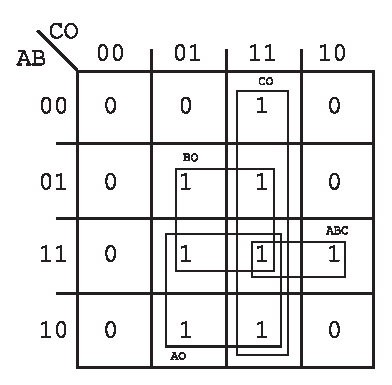
\includegraphics[height=2.0in]{kmap33db.eps}
\caption{Karnaugh Map Of 3/3 Debouncing}
\label{fig:sfrr0:svcn0:00}
\end{figure}

It can be seen from the figure that the expression for the output is

\begin{equation}
\label{eq:sfrr0:svcn0:01}
ABC + AO + BO + CO = ABC + O(A + B + C).
\end{equation}

Intuitively, (\ref{eq:sfrr0:svcn0:01}) makes sense---the output 
will be unconditionally \emph{T} if all three of the most recent samples 
are \emph{T}
($ABC$).  The output will also be \emph{T} if the previous output was \emph{T}
and at least one of the most recent samples are \emph{T} [$O(A+B+C)$]---at least
one \emph{T} recent sample blocks the output from transition to \emph{F}.

Figure \ref{fig:sfrr0:svcn0:01} supplies the C-language
code to implement 3/3 debouncing as a vertical mapping.
A C-compiler will typically implement this code very directly
using the bitwise logical instructions of the machine.

\begin{figure}
\begin{verbatim}
/**************************************************************/
/* Assume:                                                    */
/*    A      : Most recent sample (i.e. at t(0)), arranged as */
/*             a group of 8 bits.                             */
/*    B      : Next most recent sample t(-1).                 */
/*    C      : Oldest sample t(-2).                           */
/*    output : Debounced collection of 8 bits presented to    */
/*             software internals.  Note that this is both    */
/*             an input (to the combinational mapping) and    */
/*             the new result.                                */
/**************************************************************/

output = (A & B & C) | (output & (A | B | C));

/* End of code. */
\end{verbatim}
\caption{C-Language Implementation Of 3/3 Debouncing}
\label{fig:sfrr0:svcn0:01}
\end{figure}


%%%%%%%%%%%%%%%%%%%%%%%%%%%%%%%%%%%%%%%%%%%%%%%%%%%%%%%%%%%%%%%%%%%%%%%%%%%%%%%

\section{Research Interests}
\label{srin0}

This section enumerates my specific research interests.


%%%%%%%%%%%%%%%%%%%%%%%%%%%%%%%%%%%%%%%%%%%%%%%%%%%%%%%%%%%%%%%%%%%%%%%%%%%%%%%

\subsection{Mathematical Properties of Timed Automata Systems}
\label{srin0:star0}

I have interest in the mathematical properties of timed automata systems,
including these questions:

\begin{itemize}
\item Can these systems be rearranged (independent of code generation) for more 
      efficient implementation?  Is there some canonical form?
\item Can an automaton be ``factored'' into components (i.e. the reverse
      operation of ``shuffle'' illustrated in Figs. 
      \ref{fig:staf0:stfw0:00}, \ref{fig:staf0:stfw0:01}, and \ref{fig:staf0:stfw0:02})?
\item Is the factorization unique\footnote{In the same sense that the
      fundamental theorem of arithmetic guarantees that a composite
      can have only one unique factorization into primes.} 
      or can it be made unique according
      to some metric?
\item Can algorithms spot suboptimal designs and coach
      human programmers?\footnote{Example of a suboptimal design:
      identical behavior could be achieved using a simpler design.}
\end{itemize}

%%%%%%%%%%%%%%%%%%%%%%%%%%%%%%%%%%%%%%%%%%%%%%%%%%%%%%%%%%%%%%%%%%%%%%%%%%%%%%%

\subsection{Code Generation from Systems of Timed Automata}
\label{srin0:snvf0}

I have interest in the mathematics of code generation from systems of timed
automata.  One might make the observation that all of the techniques 
described in \S{}\ref{sfrr0} are individual and seemingly disjoint techniques that
come about through human ingenuity.  I am interested in:

\begin{itemize}
\item Any unified mathematical framework that includes all of the techniques.
      For example, can one find a common framework or way of thinking that includes both
      Farey series approximations and vertical counters?
\item Any mathematical framework that, given a smorgasbord of disjoint techniques,
      can predict how to apply them to obtain optimal results (this is also 
      a function of the processor instruction set).  (Cost matrices and
      least-squares methods come to mind immediately, but I'd like to examine
      this more closely.)
\end{itemize}

%%%%%%%%%%%%%%%%%%%%%%%%%%%%%%%%%%%%%%%%%%%%%%%%%%%%%%%%%%%%%%%%%%%%%%%%%%%%%%%

\subsection{Code Generation and Formal Verification of Properties in the Same Framework}
\label{srin0:sgvs0}

There seem to be no existing tools that will allow code generation (from
a timed automata model) and the
verification of formal properties in the same framework.  In addition, the tools
that do generate code (for small systems) can't optimize as effectively as a 
human programmer.  With a more sound mathematical basis for optimization,
I believe that tools should be able to optimize more effectively
than a human programmer.

%%%%%%%%%%%%%%%%%%%%%%%%%%%%%%%%%%%%%%%%%%%%%%%%%%%%%%%%%%%%%%%%%%%%%%%%%%%%%%%

\subsection{Enterprise Content Management}
\label{srin0:secm0}

I administer web-based version control and defect-tracking databases.  This type of
technology is critical because human beings don't deal well with complexity and 
there is the inherent need to serialize (one bug at a time, one change at a time, etc.).

I have some interest in enterprise content management
(see, for example, \emph{Alfresco}), especially the
buy-versus-build dilemma and the difficulty
and cost of developing custom in-house tools that are tailored to an individual
company's processes (I have some ideas in this area).


%%%%%%%%%%%%%%%%%%%%%%%%%%%%%%%%%%%%%%%%%%%%%%%%%%%%%%%%%%%%%%%%%%%%%%%%%%%%%%%
\end{document}
%
%$Log: phdtopicpropa.tex,v $
%Revision 1.20  2006/03/27 00:10:30  dashley
%Presumed final edits.
%
%Revision 1.19  2006/03/26 23:26:23  dashley
%Edits.
%
%Revision 1.18  2006/03/26 02:22:21  dashley
%Edits.
%
%End of $RCSfile: phdtopicpropa.tex,v $.

